\section{Date: 2026-09-17}
\noindent \textbf{Series ID: IIPUSASSQ} 

\noindent This series is titled U.S. Assets and has a frequency of Quarterly, End of Period. The units are Millions of Dollars and the seasonal adjustment is Not Seasonally Adjusted.The observation start date is 2006-01-01 and the observation end date is 2026-01-01.The popularity of this series is 10. \\ 

\noindent \textbf{Series ID: BSCICP035AM665S} 

\noindent This series is titled Composite Leading Indicators: Composite Business Confidence Amplitude Adjusted for Major Five Asia Economies and has a frequency of Monthly. The units are Normalised (Normal=100) and the seasonal adjustment is Seasonally Adjusted.The observation start date is 2000-02-01 and the observation end date is 2023-12-01.The popularity of this series is 1. \\ 

\subsection{Raw Regression}
\noindent Regresses the two series against each other directly. A significant result here can come just as easily from both series sharing a long-run trend as from any real relationship.

\begin{center}
\begin{tabular}{lclc}
\toprule
\textbf{Dep. Variable:}         & value\_fred\_BSCICP035AM665S & \textbf{  R-squared:         } &     0.083   \\
\textbf{Model:}                 &             OLS              & \textbf{  Adj. R-squared:    } &     0.070   \\
\textbf{Method:}                &        Least Squares         & \textbf{  F-statistic:       } &     6.363   \\
\textbf{Date:}                  &       Thu, 17 Sep 2026       & \textbf{  Prob (F-statistic):} &   0.0139    \\
\textbf{Time:}                  &           15:45:16           & \textbf{  Log-Likelihood:    } &   -123.79   \\
\textbf{No. Observations:}      &                72            & \textbf{  AIC:               } &     251.6   \\
\textbf{Df Residuals:}          &                70            & \textbf{  BIC:               } &     256.1   \\
\textbf{Df Model:}              &                 1            & \textbf{                     } &             \\
\textbf{Covariance Type:}       &          nonrobust           & \textbf{                     } &             \\
\bottomrule
\end{tabular}
\begin{tabular}{lcccccc}
                                & \textbf{coef} & \textbf{std err} & \textbf{t} & \textbf{P$> |$t$|$} & \textbf{[0.025} & \textbf{0.975]}  \\
\midrule
\textbf{const}                  &     101.6727  &        0.802     &   126.848  &         0.000        &      100.074    &      103.271     \\
\textbf{value\_fred\_IIPUSASSQ} &   -8.045e-08  &     3.19e-08     &    -2.522  &         0.014        &    -1.44e-07    &    -1.68e-08     \\
\bottomrule
\end{tabular}
\begin{tabular}{lclc}
\textbf{Omnibus:}       & 13.288 & \textbf{  Durbin-Watson:     } &    0.449  \\
\textbf{Prob(Omnibus):} &  0.001 & \textbf{  Jarque-Bera (JB):  } &   16.146  \\
\textbf{Skew:}          & -0.826 & \textbf{  Prob(JB):          } & 0.000312  \\
\textbf{Kurtosis:}      &  4.628 & \textbf{  Cond. No.          } & 1.25e+08  \\
\bottomrule
\end{tabular}
%\caption{OLS Regression Results}
\end{center}

Notes: \newline
 [1] Standard Errors assume that the covariance matrix of the errors is correctly specified. \newline
 [2] The condition number is large, 1.25e+08. This might indicate that there are \newline
 strong multicollinearity or other numerical problems.

\begin{figure}
\centering
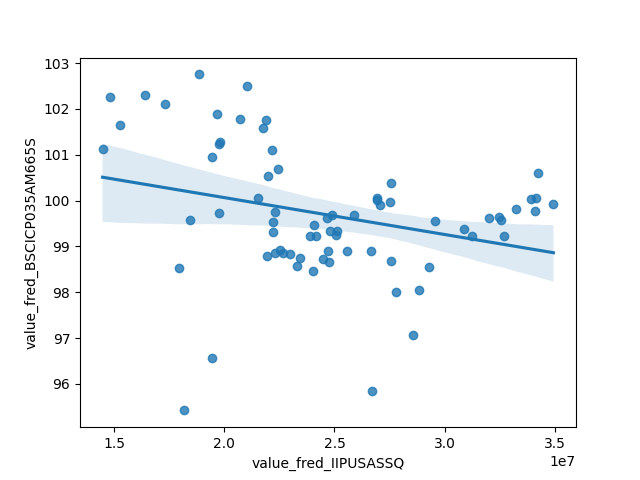
\includegraphics[scale = 0.9]{plots/plot_2026-09-17.png}
\caption{Raw Regression Plot for 2026-09-17}
\end{figure}
\newpage
\subsection{Detrended Regression}
\noindent Regresses the residuals of each series after removing its own linear time trend, so a shared trend can no longer drive the result on its own. A relationship that stays significant here is better evidence of a genuine link between the two series.

\begin{center}
\begin{tabular}{lclc}
\toprule
\textbf{Dep. Variable:}                    & value\_fred\_BSCICP035AM665S\_detrended & \textbf{  R-squared:         } &     0.178   \\
\textbf{Model:}                            &                   OLS                   & \textbf{  Adj. R-squared:    } &     0.167   \\
\textbf{Method:}                           &              Least Squares              & \textbf{  F-statistic:       } &     15.21   \\
\textbf{Date:}                             &             Thu, 17 Sep 2026            & \textbf{  Prob (F-statistic):} &  0.000219   \\
\textbf{Time:}                             &                 15:45:16                & \textbf{  Log-Likelihood:    } &   -112.66   \\
\textbf{No. Observations:}                 &                      72                 & \textbf{  AIC:               } &     229.3   \\
\textbf{Df Residuals:}                     &                      70                 & \textbf{  BIC:               } &     233.9   \\
\textbf{Df Model:}                         &                       1                 & \textbf{                     } &             \\
\textbf{Covariance Type:}                  &                nonrobust                & \textbf{                     } &             \\
\bottomrule
\end{tabular}
\begin{tabular}{lcccccc}
                                           & \textbf{coef} & \textbf{std err} & \textbf{t} & \textbf{P$> |$t$|$} & \textbf{[0.025} & \textbf{0.975]}  \\
\midrule
\textbf{const}                             &   -2.082e-12  &        0.138     & -1.51e-11  &         1.000        &       -0.276    &        0.276     \\
\textbf{value\_fred\_IIPUSASSQ\_detrended} &    3.494e-07  &     8.96e-08     &     3.900  &         0.000        &     1.71e-07    &     5.28e-07     \\
\bottomrule
\end{tabular}
\begin{tabular}{lclc}
\textbf{Omnibus:}       & 26.580 & \textbf{  Durbin-Watson:     } &    0.538  \\
\textbf{Prob(Omnibus):} &  0.000 & \textbf{  Jarque-Bera (JB):  } &   53.882  \\
\textbf{Skew:}          & -1.260 & \textbf{  Prob(JB):          } & 1.99e-12  \\
\textbf{Kurtosis:}      &  6.407 & \textbf{  Cond. No.          } & 1.54e+06  \\
\bottomrule
\end{tabular}
%\caption{OLS Regression Results}
\end{center}

Notes: \newline
 [1] Standard Errors assume that the covariance matrix of the errors is correctly specified. \newline
 [2] The condition number is large, 1.54e+06. This might indicate that there are \newline
 strong multicollinearity or other numerical problems.

\begin{figure}
\centering
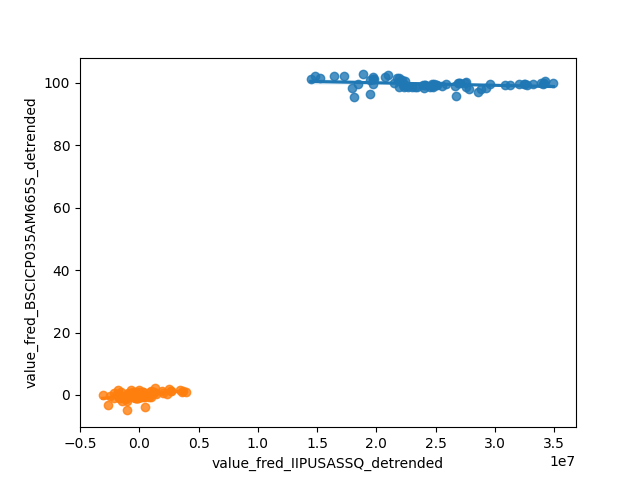
\includegraphics[scale = 0.9]{plots/plot_2026-09-17_detrended.png}
\caption{Detrended Regression Plot for 2026-09-17}
\end{figure}
\newpage
